\section{A model for on-the-spot attention and response modulation support in online conversations}~\label{sec:design}
\subsection{An Intervention for Implicit Emotion Regulation}
The majority of research in digital emotion regulation has concentrated on explicit emotion regulation, which involves a conscious effort to change one's affective state. However, as per psychological research, implicit emotion regulation is also an essential component of overall well-being \cite{gyurak2011explicit}, \cite{braunstein2017explicit}. While explicit emotion regulation requires conscious effort to initiate and monitor during implementation and is associated with some level of insight and awareness, implicit emotion regulation is elicited automatically by the stimulus itself and runs to completion without monitoring and can occur without insight and awareness. Habitual emotion modification, in which a person performs emotion regulation to routinely achieve a specific goal, is an example of implicit emotion regulation \cite{gross2006emotion}. 
Currently, the digital tools available to assist ER are based on the user's need; thus, they not only require their users to be aware that they are attempting to change their affective state but also to choose appropriate tools to do so. Scrolling through social media applications to escape participating in a situation is one such example of digital emotion regulation where the user is although habitually scrolling but is aware of the platform. As a result, we believe that by emphasising instances of intense emotional expression and reactions, we can make emotionally charged elements clear and easy to perceive, which, when encountered repeatedly, will trigger habitual emotion regulation.
\subsection{Proposed methodology}
The proposed framework for encouraging emotion regulation in social media conversations is depicted in Figure-\ref{fig:Framework}. It is composed of three key components: data retrieval, emotion propagation analysis, and emotion regulation recommendations. The data retrieval process starts with gathering information from social media conversations, in this case Twitter conversations. In recent years, Twitter has been a popular destination for hashtag-based social movements such as \#MeToo and \#BlackLivesMatter, but the platform's free speech policy also increases the risk of hate and harassment. Therefore, we gathered a variety of Twitter conversations and saved them as CSV files. We used feature engineering to create a set of files, each containing a conversation wherein each row comprised of a text string representing a tweet or a comment, as well as their ID and metadata (parameters like the number of comments received, authors who replied etc). The second component then analyses emotion propagation using these CSV files. It begins with categorising the emotions expressed in tweets. Emotions are divided into 6 primary and 27 secondary groups. We use the primary emotion categories in this work to classify the emotion in tweets. We generate a graph of the conversation after classifying the tweets into 6 emotion classes. This graph is used to calculate the emotional impact of individual tweets on the entire conversation as well as the percentage distribution of various emotions in the discussion. Following that, in the final component, we use the graph to identify the nodes that have the greatest impact on the emotion of the conversation and apply this information to identify scenarios where emotion regulation needs to be undertaken and offer support for the same.
\begin{figure}[h]
  
    \centering
    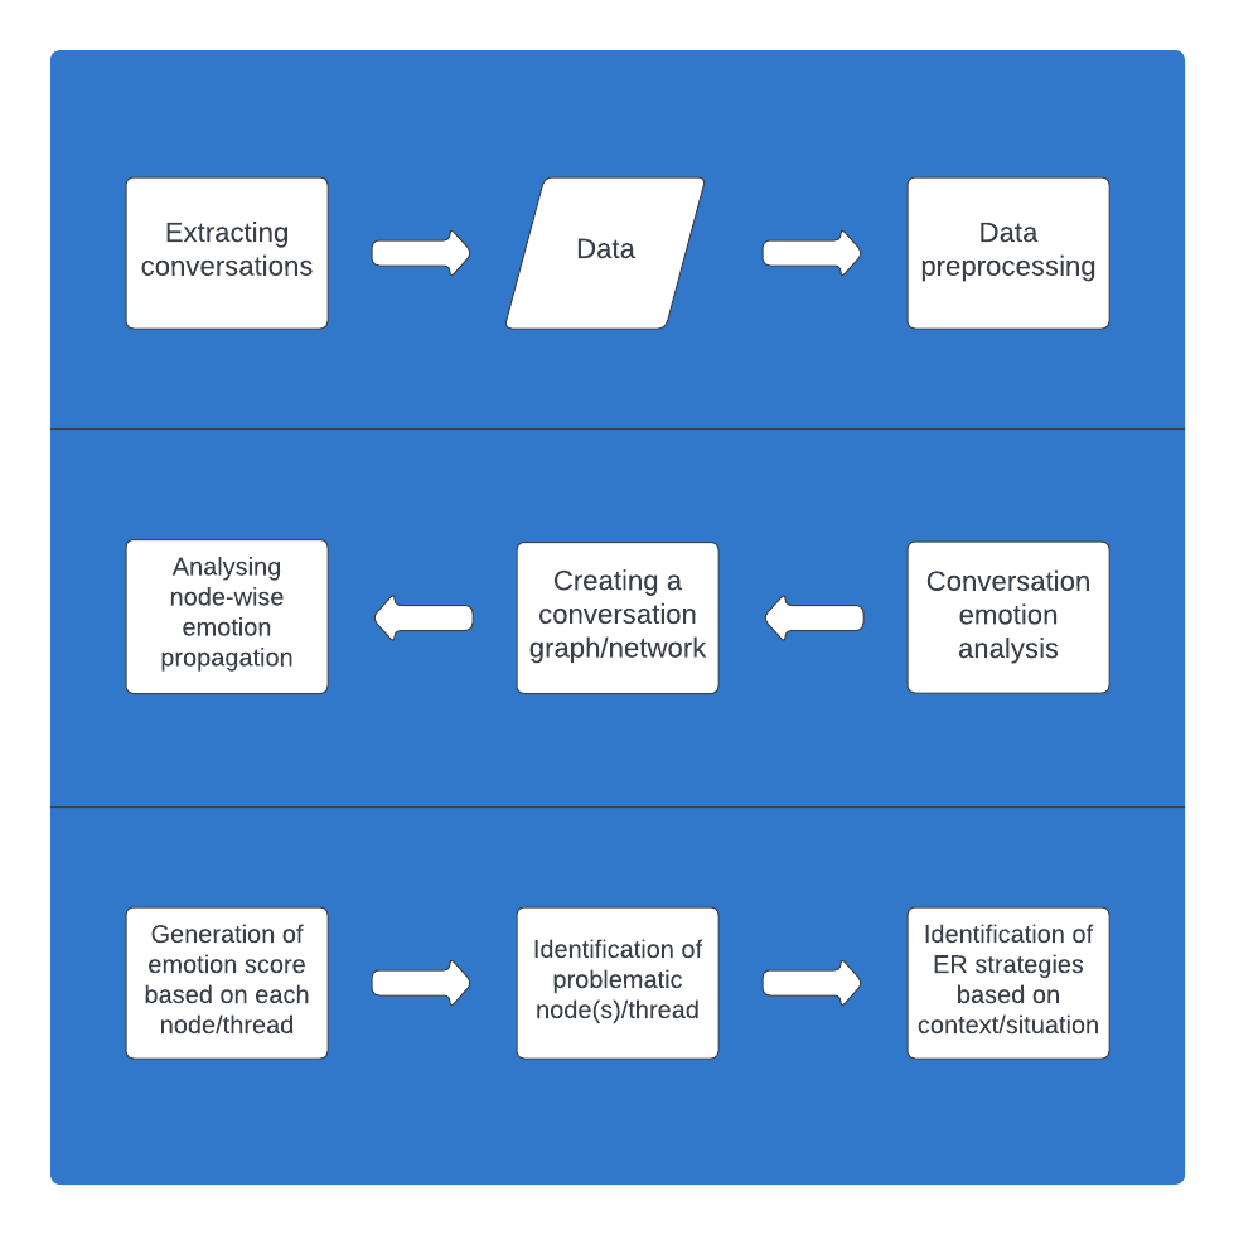
\includegraphics[width=12cm,height=12cm,keepaspectratio]{framework.pdf}
%   \includegraphics[width=5cm,height=5cm,keepaspectratio]{samples/sample_convv.png}
%   \includegraphics[width=5cm,height=5cm,keepaspectratio]{samples/sample_conv_graphh.png}
  \caption{Framework for encouraging on-spot emotion regulation in social media conversations}
  \label{fig:Framework}
  \end{figure}  
%%%%%%%%%%%%%%%%%%%
\subsection{Experimental Evaluation and Analysis}

 

